\documentclass[11pt,a4paper]{jsarticle}
\usepackage[dvipdfmx]{graphicx}
\usepackage{url}

\title{日本におけるデジタル化の状況}
\author{G685052026 森田 伊織}
\date{2026年7月13日}

\begin{document}

\maketitle

\section{デジタル競争力ランキング}
国際経営開発研究所 (IMD) の調査 \cite{imd} によると，日本のデジタル競争力のランキングは図 \ref{fig:ranking} に示すように，調査対象の 64 カ国中，総合で 28 位，知識分野で 25 位となっている．

\begin{figure}[htbp]
    \centering
    % 1枚目の画像ファイル名（例: fig31.png または適切なファイル名に変更してください）
    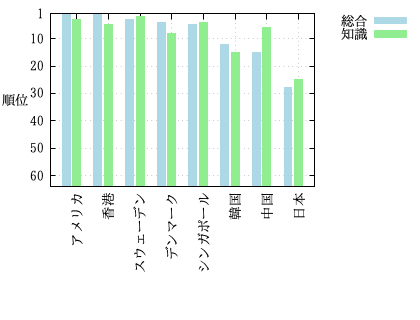
\includegraphics[width=0.7\textwidth]{fig31.png}
    \caption{デジタル競争力ランキング (64 カ国中)}
    \label{fig:ranking}
\end{figure}

\section{ブロードバンドの整備状況}
OECD によるブロードバンド回線の普及に関する調査 \cite{oecd} によると，表 \ref{tab:broadband} に示すように，日本における 100 人あたりの光ファイバー回線の加入者数は 29.0 で，韓国，スウェーデン，ノルウェーに続いて第 4 位になっている．

\begin{table}[htbp]
    \centering
    \caption{光ファイバー回線の加入者数 (100 人あたり)}
    \label{tab:broadband}
    \begin{tabular}{|c|l|r|}
        \hline
        順位 & 国名 & 加入者数 \\ \hline
        1 位 & 韓国 & 38.2 \\ \hline
        2 位 & スウェーデン & 31.9 \\ \hline
        3 位 & ノルウェー & 29.5 \\ \hline
        4 位 & 日本 & 29.0 \\ \hline
        5 位 & アイスランド & 28.8 \\ \hline
        6 位 & スペイン & 27.3 \\ \hline
        7 位 & ポルトガル & 25.1 \\ \hline
        8 位 & ニュージーランド & 23.6 \\ \hline
        9 位 & リトアニア & 22.3 \\ \hline
        10 位 & フランス & 21.2 \\ \hline
    \end{tabular}
\end{table}

\section{考察}



\begin{itemize}
    \item 図１などと書くときにコードを使うのは後から図を加えて順番がずれても自動で直してくれるようにするため。
    \item width=10cm のようにしないのは、0.7 のようにパーセントで指定しておくと、後からページの余白や紙のサイズ（A4からB5など）を変えたときでも、画面からはみ出すことなく自動的に丁度いいバランスで縮小・拡大されるためである。
\end{itemize}

\begin{thebibliography}{9}
\bibitem{imd}
IMD. IMD world digital competitiveness ranking. \url{https://www.imd.org/centers/world-competitiveness-center/rankings/world-digital-competitiveness/}, 2021.

\bibitem{oecd}
OECD. Broadband Portal. \url{https://www.oecd.org/digital/broadband/broadband-statistics/}, 2022.
\end{thebibliography}

\end{document}